\documentclass{beamer}

\usepackage[T2A]{fontenc}
\usepackage[utf8]{inputenc}
\usepackage[russian]{babel}


\hypersetup {
    unicode = true
}

\usetheme{Madrid}
\usecolortheme{whale}

\title[Инструментальная среда]
{Инструментальная среда для анализа программных систем}
\author[А.М. Половцев]{
    А.М. Половцев гр. 63501/13\\
    Руководитель: Ицыксон В.М.\\
    Аттестация №3
}
\date[28.02.2013]{}

\begin{document}

\frame{\titlepage}

\begin{frame}
\frametitle{Архитектура инструментального средства}

\begin{figure}[h!]
    \begin{center}
        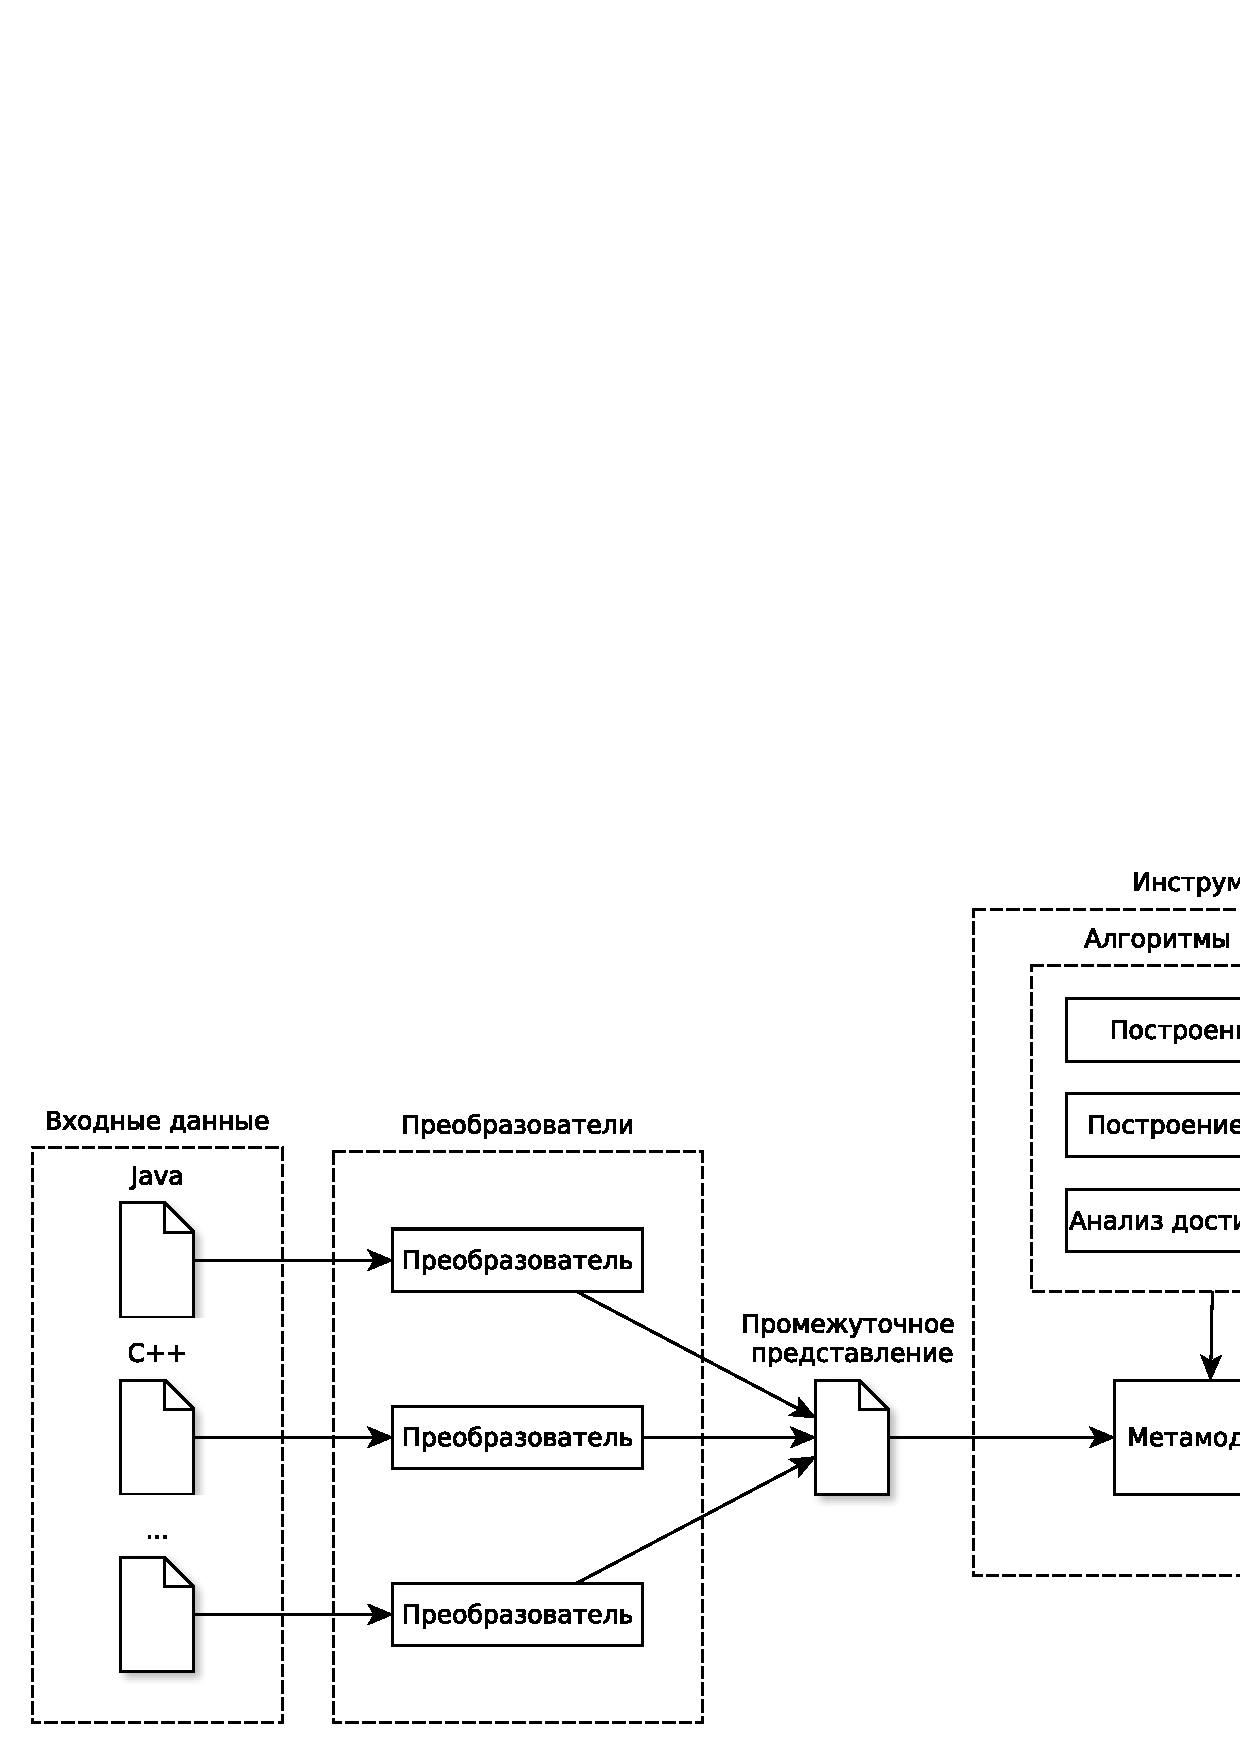
\includegraphics[width=\textwidth]{img/architecture.png}
    \end{center}
\end{figure}
\end{frame}

\begin{frame}
\frametitle{Что было сделано}
    \begin{itemize}
        \item[\checkmark] Написан простой парсер языка Java
        \item[-] Реализация обратного преобразования из xml в Java
    \end{itemize}
\end{frame}

\begin{frame}
\frametitle{Спасибо за внимание}
\center{\resizebox{60pt}{80pt}{?}}
\end{frame}

\end{document}
